\section{Specification}
\label{sec:specification}

In accordance with the selected methodology of Use Case 2.0 (see \autoref{sec:design}) no in-depth specification has been written, however a reasonable amount of \glspl{use_case} has been defined and iterativly refined. These were then reviewed by the client and discussed in detail. All \glspl{use_case} have been described on cards on Trello and \glspl{use_case_slice} have been generated out of those. They are directly reflected by the description in \cite{sassoon2016,sassoon2014, sassoon2016CD}. In general each \gls{use_case} consists of the following attributes: Name, Desired outcome, (Main-)\Glspl{Actor}, Flow to achieve the desired outcome, and Alternative flow (optional).


\subsection{Weak Requirements}
\label{sub:weak}
In addition to the described \glspl{use_case} in \autoref{tab:usecases} (derived from \autoref{sub:aims}), the following weak requirements influenced the development of the final project:


\begin{itemize}
	\item The system should be designed as an interactive \textbf{web application} to ensure:
	\begin{itemize}
		\item Access for multiple users.
		\item Portability between different operating systems.
		\item No requirement of installation of software on local computers.
		\item Clinician and statistician can share the same infrastructure without the need of working at the same place.
	\end{itemize}
	\item A decent test suite should be provided to ensure the functionality of the system.
	\item The system must be suitable for different user types (\glspl{Actor}).
	\item The system has to provide different levels of access for different user groups.
	\item The system has to execute test scripts as \gls{R}-Scripts.
	\item The system should be hosted on a free accessible hosting provider.
\end{itemize}


\subsection{Actors in our System}
\label{sub:sassoon:actors}
During the requirements analysis the following actors have been identified and are described as follows:

\textbf{Clinicians} are the main users of the system and do the actual analysis of a data set by using the predefined research questions, models and assumptions. A clinician should see all globally available research questions, models and their assumptions. In addition the preferences defined by the statistician will apply to all analyses a clinician performs. However, they will be able to enter personal preferences between models that only apply for their analyses. An overview over those \glspl{use_case} can be seen in \autoref{fig:usecase:clinician}.

\textbf{Statisticians} are able to enter statistical models into the system and to define global applicable preferences. To do so, a statistician can enter different types of assumptions mapped to models and preferences. These might contain query assumptions, where the clinician performing an analysis has to confirm a fact, or test assumptions that are checked against the data set by running an \texttt{R}-script. A statistician is as well allowed to see all data sets that have been uploaded and to check which analysis have been performed (see \autoref{fig:usecase:statistician}).



\textbf{Administrators} are able to create, modify and delete all available data in the system. In addition an administrator is required to approve new users and to assign them to a role. They are as well capable of inviting new users into the system. An overview over their \glspl{use_case} can be seen in \autoref{fig:usecase:admin}.





\subsection{Use Cases}
\label{sub:use_cases}
\autoref{tab:usecases} shows an overview over the major \glspl{use_case} being generated during the requirements analysis. For the sake of simplicity they have not been integrated into this thesis. However, they are available on the \href{https://trello.com/b/ywCkicpc}{Trello-Board}\footnote{\url{https://trello.com/b/ywCkicpc}}.

The \glspl{use_case} defined in \autoref{tab:usecases} were then further defined, deriving requirements have been generated as \glspl{use_case_slice} and were implemented by applying an iterative approach. Close feedback loops to the author of \cite{sassoon2016,sassoon2014,sassoon2016CD} (\gls{product owner} or client) ensured the correctness of these implementations. As the software was developed in a test driven approach (see \autoref{sec:tdd}), all features were implemented by designing tests first. This is reflected by the final test suite (see \autoref{sub:test_suit}) which contains a decent amount of \glspl{unit_test}, \glspl{integration_test} and \glspl{e2e_test} and has an overall test coverage of $ \geq 85\%$\footnote{\url{https://codeclimate.com/github/sebastianzillessen/small-data-analyst/coverage}}. \autoref{uc:121} shows an exemplary, detailed description of one \gls{use_case}.

\begin{landscape}
	\begin{longtable}{ l l p{11cm} l l p{3cm} }
		\textbf{ID}                         & \textbf{\Gls{Actor}}\footnote{C: Clinician, S: Statistician, A: Admin} &\textbf{Description} &  \textbf{RC} & \textbf{Prio}\footnote{MoSCoW priorities} &  \textbf{Comments}\\
		\href{https://trello.com/c/KEOokZp9}{UC1}   & 	- & 	Enter two default models into the system as code without user interface including definition of assumptions & RC1 & Must &  For initial testing purposes  \\
		\href{https://trello.com/c/ebVrFdA5}{UC2}   & 	C & 	Get models that are appropriate for a research question & RC1	& Must &	   \\
		\href{https://trello.com/c/ORRBjISQ}{UC2-1} & 	C & 	Store finished analyses & RC2 & Should &  see \autoref{as:1} \\
		\href{https://trello.com/c/qKLAoWRj}{UC3} 	&  	S & 	Define assumptions for models & - & - & obsolet \\
		\href{https://trello.com/c/7NINsfz8}{UC4}   & 	C & 	Check that a data set meets the set of assumptions of a model and that the queries to the clinician regarding the research question's  assumptions are met as well & RC1 & Must   &   \\
		\href{https://trello.com/c/22JGne3r}{UC5}   & 	C & 	Select a research question & RC1 & Must &   \\
		\href{https://trello.com/c/CVGBVWID}{UC6}   &   C, S, A & 	Login into the system and be authenticated with your role & RC2 & Should &	 \\
		\href{https://trello.com/c/pId27kJM}{UC6-1} &   A & 	Create new users & RC2 & Must &	 \\
		\href{https://trello.com/c/pQ98qgSL}{UC6-2} &  	A & 	Delete users & RC2 & Must	 &   \\
		\href{https://trello.com/c/mvxBeNSR}{UC6-3} &  	A & 	Modify users & RC2 & Should &   \\
		\href{https://trello.com/c/DidVQKAS}{UC7}   &   C & 	Fill patient data into the system to be checked by the models & RC2 & Must &  \\
		\href{https://trello.com/c/be2088JH}{UC8}	& 	C & 	Inspect arguments for and against models for a research question & RC2 & Must &   \\
		\href{https://trello.com/c/Ca9mA3uA}{UC9}   &   C & 	Define new personal preferences & RC3 & Must &   \\
		\href{https://trello.com/c/Ca9mA3uA}{UC9-1}   &   S & 	Define new global preferences & RC3 & Must &   \\
		\href{https://trello.com/c/1s656fA9}{UC10}  &   C & 	Get recommended model taking into account global preferences & RC3 & Should & 	 \\
		\href{https://trello.com/c/xUDStSOK}{UC11}  &   A & 	Create new users with a specific role for the system & RC3 & Could &    \\
		\href{https://trello.com/c/5UMo7o6U}{UC12}  &   S & 	Enter additional analysis models into the system in a defined language as text so that it will be regarded as an option for applicable models	& RC3 & Should & \\
		\href{https://trello.com/c/2V6Cl65u}{UC12-1}&   S & 	Add Test-Argument into the system & RC2 & Must & \\
		\href{https://trello.com/c/OwM2Z7wt}{UC12-2}&   S & 	Add Query-Argument into the system & RC2 & Must &  \\
		\href{https://trello.com/c/VThxB5aS}{UC12-3}&   S & 	Add Test-Query-Assumptions into the system & RC4 & Should & added later\\
		\href{https://trello.com/c/CkpJUNPW}{UC12-4}&   S & 	Run Test-Argument on a specific existing data set & RC3	& Should &  \\
		\href{https://trello.com/c/Rg6GPnNE}{UC12-5}&   S & 	Add Blank Arguments for grouping of assumptions & RC2 & Could & \\
		\href{https://trello.com/c/ORlMByiQ}{UC13}  &   S & 	Get in-depth information about algorithmic performance & RC4 & Would & rejected\\
		\href{https://trello.com/c/NcV3lo4w}{UC14}  &   C & 	Enter personal preferences for statistical models and/or analysis techniques & RC4 & Could &   \\
		\href{https://trello.com/c/BOUu2hKN}{UC15}  &   C & 	Inspect argumentation frameworks that are generated for/against the statistical models. Graph Export: See arguments for and against models for a research question in a nice and graphical &RC4 & Would & 	 ignored as printing of generated graphs possible  \\
		\href{https://trello.com/c/3FCcFdmm}{UC16}  &   C & 	Inspect analysis process of argumentation framework as visualisation & RC4 & Would	&    \\
		\href{https://trello.com/c/Hv2xe2UW}{UC17}  &   S & 	Enter additional research questions into the system & RC3 &Could& \\
		\href{https://trello.com/c/w1YiIgU7}{UC17-1}&   S & 	Modify research questions&RC3 & Must &  \\
		\href{https://trello.com/c/UbT5mtDx}{UC17-2}&   S & 	Delete research questions&RC3&Must& \\
		\href{https://trello.com/c/dpLHOxbB}{UC18}  &   S & 	Include R-script execution	 & RC1 & Must & \\
		\href{https://trello.com/c/bZHdWpkt}{UC19}  &   S & 	Enter global preferences for statistical models and/or analysis techniques& RC3 & Could &	 \\

		\caption{List of the different use cases being defined during the requirements analysis.}	
		\label{tab:usecases}
	\end{longtable}
\end{landscape}



{ \tiny
	\begin{longtable}{|p{2cm} p{11cm}|}

		\hline
			\textbf{ID} & 
				\href{https://trello.com/c/2V6Cl65u}{UC12-1}\\
			
			\hline
			\textbf{Actor} & Statistician or Admin \\
			\hline
			\textbf{Description} & 
				Add Test-Argument into the system\\
			\hline
			\textbf{Desired~outcome} & 
				- A statistician can create new arguments \newline
				- These arguments can be assigned to models \newline
				- The arguments are accessible for all users in the system \newline
		\\
		\hline
			\textbf{Flow} & 
				1.) The user is logged in as Admin/Statistician  \newline
				2.) The User clicks on "Add Test-Argument" (see \href{https://trello.com/c/OwM2Z7wt}{Query arguments}, \href{https://trello.com/c/Rg6GPnNE/39-uc12-5-add-attacks-between-arguments}{Blank arguments})\newline
				3.) The system shows a form including "Name", "Description", "Attacking (Model or Other Argument)", "Required data set fields", "R-Code to run test" and a disabled submit button\newline
				4.) The User enters a Name\newline
				5.) The user might enter a description\newline
				6.) The User selects at least on Model or other Argument from the list of possible attacked objects and whether it is critical or non-critical to that object.\newline
				7.) The user enters a list of required data set fields.\newline
				8.) The user enters the R-Code to test if this argument holds or not. The R-Code must return a true/false statement at the end, \texttt{True} saying the argument holds, otherwise \texttt{False}. The R-Script will get as input a variable named \texttt{tabular\_data}  and must assign the variable \texttt{result} with \texttt{true} / \texttt{false} (see \autoref{sec:r_code}). The attributes specified in "Required data set fields" will be checked before executing the \texttt{R}-Script.\newline
				9.) The user is in charge of verifying his script against data sets. A functionality to do so will be given by selecting a data set in the system first. The script will then be checked against this data set.\newline
				10.) The user clicks submit. The system performs a validation of the argument.\newline
				11.) The System stores the argument in the database and redirects the user to a list of available arguments and shows a success message.
		\\
		\hline
			\textbf{Alternatives} & 
							1.a) Not logged in as Admin: No changes to arguments possible.
				\newline	4.a) No name entered: show required inline message, disable submit button.
				\newline	6.a) No attacked object selected: show required inline message, disable submit button.
				\newline	8.a) If the user does not enter a R-Script: mark as required and do not enable submit button.
				\newline	9.a) If there is a syntax error: Show syntax error and line to the user
				\newline	9.b) If the result is not boolean: Show error explaining true/false result required.
				\newline	9.c) If there has been an error during execution with the test data set: show error.
				\newline	9.d) After successful run: Show the data set used to test it and the result.
				\newline	10.a) If the user does not select "Submit": NO changes done.
				\newline	11.a) If the validation fails: Redirect the user back to the form page and show validation failure.
				\newline	11.b) If any error occurs,  Redirect the user back to the form page and show error explanation.
							\\
		\hline

	\label{uc:12-1}\\
	\caption{Use case 12-1: "Add Test-Argument into the system." An example for a detailed description of a use case.}
\end{longtable}
}



\subsection{Technical Specification}
\label{sub:technical}

As the system should be accessible by multiple users and from different departments (e.g. clinicians and statisticians), it will be developed as a web-application in \gls{RoR}\footnote{\url{http://rubyonrails.org}} and will be hosted on Heroku\footnote{\url{https://www.heroku.com}} as this will provide an easy-to-use and easy-to-deploy environment. In addition it allows us to host the demo application for free. To provide a \gls{CI} environment, the project code is hosted on \texttt{github}\footnote{\url{https://github.com/sebastianzillessen/small-data-analyst}} and a \texttt{Travis CI}\footnote{\url{https://travis-ci.org/sebastianzillessen/small-data-analyst}} instance has been setup that runs all the implemented tests of the project.

The used data sets are anonymised, so data protection issues are reduced to a minimum and the data sets can be hosted in the cloud. \texttt{PostgreSQL}\footnote{\url{http://www.postgresql.org}} will be used as a database, as it is well integrated on Heroku and provides high scalability. Generated plots are stored in an Amazon Web Services S3 Storage\footnote{\url{https://aws.amazon.com/s3}, a simple storage service.}.

The assumption tests for the statistical models will be performed in \gls{R}, as this is a common used language for statistical calculations and well known by statisticians. In addition many assumption-checks already exist in \gls{R}. These scripts (externally provided) will be executed in the \gls{RoR} application with the help of third party gems. A detailed description of this process can be found in \autoref{sec:r_code}.

To provide a responsive and clear user interface the \texttt{Bootstrap}\footnote{\url{http://getbootstrap.com}} framework will be used to design and style the application. 

\subsection{Data Flow in the System}


\autoref{fig:data_flow} shows the simplified data flows in the process of statistical model selection: First of all, the statistician has to create research questions (1) including their possible models (2) and the required assumptions (3) and global preferences (4). These are all stored in a knowledge base which is itself stored in  a persistent database. A detailed description of all database classes can be found in \autoref{sub:db}. 

\begin{figure}[btph]
	\centering
	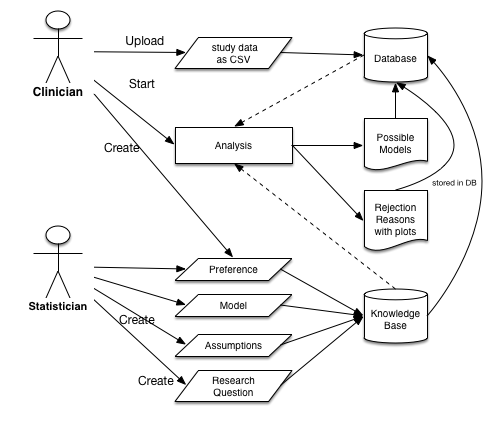
\includegraphics[width=0.8\textwidth]{figures/data_flow}
	\caption{Core data flow in the system to create new analyses.}
	\label{fig:data_flow}
\end{figure}


A clinician can upload new clinical data retrieved from studies by using the CSV upload functionality (6). Starting a new analysis (7) retrieves the data set from the database and instantiates the knowledge base for this specific problem. The assumptions of all applicable models for the selected research question are then evaluated. If multiple models are possible, the preferences (first the globally defined ones by a statistician, later the personal preferences (5) a clinician might have) are applied in order of there importance until one last model remains. This model is then returned as recommended model. The process of the rejection of various models will be graphically visible to the user (see \autoref{sub:ui}). The process of creating and processing a new analysis is described in detail in \autoref{sub:walk}.


